\documentclass{article}
\PassOptionsToPackage{numbers}{natbib}
\usepackage[final,sglblindworkshop]{neurips_2026}
\usepackage[utf8]{inputenc}
\usepackage[T1]{fontenc}
\usepackage{
  hyperref,url,booktabs,tabularx,amsfonts,amsmath,
  microtype,xcolor,graphicx,tikz
}
\usetikzlibrary{positioning,arrows.meta,calc}
\hypersetup{hidelinks}
\workshoptitle{Galileo Hackathon 2026}

\makeatletter
\renewcommand{\@noticestring}{
  Galileo Hackathon 2026. Participant research report.
}
\makeatother

\newcommand{\interp}[1]{\emph{Interpretation: #1}}
\newcommand{\Cn}{C$_{\rm nmse}$}
\newcommand{\Bn}{B$_{\rm nmse}$}
\newcommand{\Ce}{C$_{\rm ens}$}

\title{Validation can't see extrapolation: symmetry, data and periodicity in wake forecasting}
\author{
  Team Optimus (Raghav Vijayakannan, Pranav Vijay Krishna, Hrithik Yash)\\
  Team ID: G2-12 \quad Task: pitching-wing-wake
}

\begin{document}
\maketitle

\begin{abstract}
Forecasting the wake of a pitching airfoil has two different limits: learning the
dynamics inside the training range, and extrapolating beyond it. They need
different fixes, and the public validation set measures only the first. Training
changes (reflection augmentation and averaging, more data, a variance-normalised
loss, a two-network ensemble) lowered validation NMSE from 0.2571 to 0.1181
($-54\%$). A parameter-free copy of the history by whole forcing periods left
validation unchanged (0.1440) yet gave our largest single portal drop, from 0.2876
to 0.1789. Overall the
final portal score fell from the organizer baseline's 0.3937 to 0.1538 (\#129,
$-61\%$). Validation and the hidden
extrapolation tiers measure different things: training cut validation error by
54\%, yet our largest hidden-score drop came from a physics-based period copy that
validation could not see.
\end{abstract}

\section{Scientific goal \& initial hypothesis}

We forecast 20 vorticity frames behind a pitching NACA0012 ($Re=500$) from 10 past
frames and the pitching frequency $k$ and amplitude $\theta_0$. Our starting
question was whether teaching or enforcing the problem's reflection symmetry
improves forecasts at unseen conditions. Reflection consistency means that
reflecting the input reflects the predicted wake; an individual wake need not be
symmetric. For $y\mapsto-y$, $G$ negates the history's vorticity, reverses its rows
and negates the pitch-phase sine and cosine ($k$, $\theta_0$ unchanged); $S$
negates and reverses the forecast. Averaging a predictor $F_B$ gives
\begin{equation}
F_C(x)=\tfrac12\left[F_B(x)+S F_B(Gx)\right],
\end{equation}
reflection-consistent by construction at the cost of two passes. We hypothesised
that augmentation would reduce inconsistency and averaging remove it and improve
accuracy; lower inconsistency without lower error would contradict this. The hidden
test adds a regime-boundary band (T2) and amplitude and frequency extrapolation (T3a,
T3f), while all 12 validation cases lie inside the training range
(Fig.~\ref{fig:setting}a). This made a second question the main one: which
improvements can validation detect?

\begin{figure}[!ht]
\centering
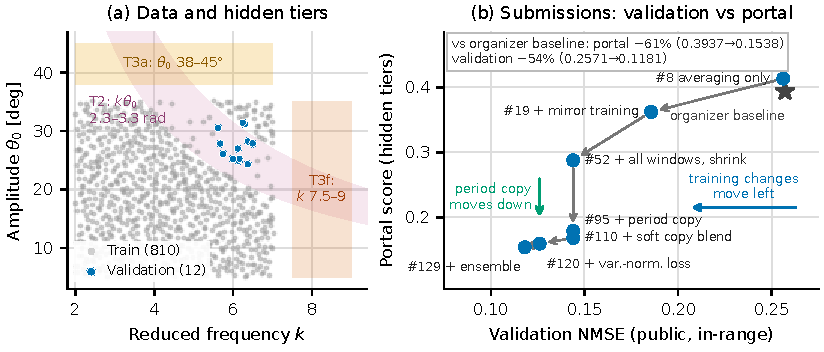
\includegraphics[width=\linewidth]{figures/fig1_setting.pdf}
\caption{(a) Training and validation conditions and the hidden tiers. Only one
coordinate of T3a ($\theta_0$) and T3f ($k$) is published; shading spans the
training range of the other. (b) Each submission's validation NMSE against its
portal score, in submission order; \#129 is the final submission (0.1538).}
\label{fig:setting}
\end{figure}

\section{Research trajectory}

Averaging the organizer checkpoint (A$_{\rm ref}$) barely changed validation, so we
trained B with reflection augmentation and averaged it (C). C's portal score (0.3620)
was far above its validation NMSE, so we built proxies from training data (train on
$k\le5.5$, score $k$ 6--7; train on $\theta_0\le30^\circ$, score 31--35$^\circ$); they
showed the network failing beyond its training frequencies and led to the shrinkage
and the period copy. In parallel we used all 68,040 training windows instead of
22,680 (B+), a variance-normalised loss (\Bn) and a two-network ensemble (\Ce). In
Fig.~\ref{fig:setting}b training changes move points mainly left, while the period copy
moves them straight down with no validation change (Table~\ref{tab:traj}).

\begin{table}[h]
\centering
\footnotesize
\setlength{\tabcolsep}{4pt}
\begin{tabular}{@{}llrl@{}}
\toprule
Submission & Change & Validation & Portal (\#)\\
\midrule
C\_on\_A & averaging on organizer weights & 0.2562 & 0.41326 (\#8)\\
C\_from\_B & + reflection-augmented training (B) & 0.1856 & 0.36196 (\#19)\\
C\_from\_Bplus\_ood & + all windows (B+), out-of-range shrink & 0.1440 & 0.28762 (\#52)\\
C\_from\_Bplus\_hybrid & + period copy, hard gate & 0.1440 & 0.17894 (\#95)\\
C\_from\_Bplus\_hybrid2 & + soft copy blend for $k>7$ & 0.1440 & 0.16798 (\#110)\\
C\_nmse\_hybrid & + variance-normalised loss (\Bn) & 0.1261 & 0.15930 (\#120)\\
C\_ens\_hybrid & + 0.6\,\Cn{} / 0.4\,C+ ensemble & 0.1181 & 0.1538 (\#129)\\
\midrule
Width 96 (rejected) & 1/3 windows, 30 ep.; all, 10 ep. & 0.1463; 0.1382 & not submitted\\
3-network mix (rejected) & 0.4 width-96 (all) + 0.4 \Cn{} + 0.2 C+ & 0.1161 & not submitted\\
\bottomrule
\end{tabular}
\caption{Submissions. Shrinkage and copy never trigger on validation, so rows 3--5
share 0.1440. Portal: hidden tiers, lower is better; baseline 0.3937.}
\label{tab:traj}
\end{table}

\section{Final model \& comparisons}
\label{sec:final}

Against the organizer baseline, the final model lowers validation NMSE from
0.2571 to 0.1181 ($-54\%$), and our final portal score is 0.1538 against 0.3937
($-61\%$).

\begin{center}
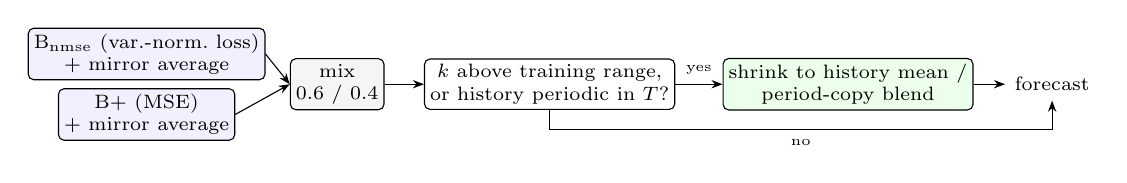
\begin{tikzpicture}[font=\scriptsize, >={Stealth[length=4pt]},
  box/.style={draw, rounded corners=2pt, align=center, inner sep=2pt, fill=#1}, box/.default=white]
\node[box=blue!6] (n1) {\Bn{} (var.-norm.\ loss)\\+ mirror average};
\node[box=blue!6, below=1mm of n1] (n2) {B+ (MSE)\\+ mirror average};
\coordinate (m) at ($(n1.east)!0.5!(n2.east)$);
\node[box=gray!8, anchor=west] (mix) at ($(m)+(5mm,0)$) {mix\\0.6 / 0.4};
\node[box, anchor=west] (q) at ($(mix.east)+(5mm,0)$) {$k$ above training range,\\or history periodic in $T$?};
\node[box=green!8, anchor=west] (fix) at ($(q.east)+(6mm,0)$) {shrink to history mean /\\period-copy blend};
\node[anchor=west] (out) at ($(fix.east)+(4mm,0)$) {forecast};
\draw[->] (n1.east) -- (mix.west); \draw[->] (n2.east) -- (mix.west);
\draw[->] (mix) -- (q); \draw[->] (q) -- node[above, font=\tiny]{yes} (fix); \draw[->] (fix) -- (out);
\draw[->] (q.south) |- ($(q.south)+(0,-2.5mm)$) -| node[pos=0.25, below, font=\tiny]{no} (out.south);
\end{tikzpicture}
\end{center}

\textbf{Final model (\#129).} Two width-64 U-Nets (1,890,708 parameters each),
seed-0 released initialization, reflection augmentation ($p=0.5$), all 68,040
windows of the 810 training cases, 40 epochs; B trained in 1,068\,s, B+ in 3,882\,s,
\Bn{} in 4,468\,s on one H100. The 0.6/0.4 weight was fixed
without a recorded search and evaluated only on validation, so 0.1181 is not an
independent estimate.

\begin{table}[h]
\centering
\footnotesize
\begin{tabular}{@{}lrrr@{\qquad}lrrr@{}}
\toprule
Model & NMSE & Final lead & Defect & Model & NMSE & Final lead & Defect\\
\midrule
A$_{\rm ref}$ (organizer) & 0.2571 & 0.4105 & 0.1638 & C+ & 0.1440 & 0.2121 & 0\\
A$_{\rm avg}$ & 0.2562 & 0.3696 & 0 & \Bn & 0.1526 & 0.2206 & 0.0469\\
B & 0.2094 & 0.3144 & 0.0505 & \Cn & 0.1261 & 0.1837 & 0\\
C & 0.1856 & 0.2754 & 0 & \Ce{} (final) & \textbf{0.1181} & \textbf{0.1747} & 0\\
B+ & 0.1670 & 0.2373 & 0.0493 & E (A$_{\rm ref}$+B mean) & 0.1897 & 0.2855 & --\\
\bottomrule
\end{tabular}
\caption{Validation (official scorer: per-lead NMSE clipped at 4, then averaged).
Defect: reflection inconsistency. \Ce{} passes the output, finiteness, NMSE$\le$1 and
non-frozen-forecast checks; batch-1 latency 88.2\,ms on one laptop CPU thread
(limit 100\,ms; GPU latency not measured).}
\label{tab:val}
\end{table}

Intervals: 2,000 resamples of the 12 paired case means (seed 0; case sampling, not
seed variation). \textbf{Averaging after mirror
training} improves all 12 cases ($-0.0238$ $[-0.0273,-0.0204]$), while averaging
the organizer weights is inconclusive ($-0.0010$ $[-0.0717,0.0585]$).
\textbf{More windows}: C+ $-$ C $=-0.0416$
$[-0.0475,-0.0362]$, 12/12, at about three times the training steps.
\textbf{Variance-normalised loss}: \Cn{} $-$ C+ $=-0.0179$ $[-0.0304,-0.0044]$, 8/12. \textbf{Ensemble}:
\Ce{} $-$ \Cn{} $=-0.0080$ $[-0.0123,-0.0043]$, 10/12.

\begin{figure}[!ht]
\centering
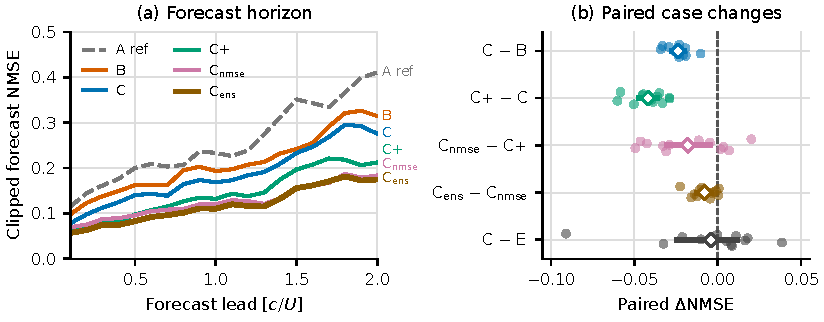
\includegraphics[width=\linewidth]{figures/fig2_accuracy.pdf}
\caption{(a) Case-averaged clipped NMSE per lead. (b) Paired per-case changes; dots
are cases, diamonds means, bars 95\% case-bootstrap intervals; negative favours the
first model.}
\label{fig:accuracy}
\end{figure}

\textbf{Extrapolation and period copy.} On the frequency proxy the averaged CNN
scored 0.99. The forcing period $T=2\pi/k$ is known, so the forecast can copy the
history forward by whole periods, gated by how well the history repeats with
period $T$ (normalised residual $r$). With the history lengthened to one period,
1,944 of 2,100 training windows (523 cases, $k$ 3.5--7) pass $r<0.3$ with mean NMSE
0.059, and periodic windows score 0.044--0.058 in every $k$ bin. With the real
10-frame history it applies only for $k\ge6.98$ (Fig.~\ref{fig:copy}). Copying commutes with $S$, so consistency is kept.

\begin{figure}[!ht]
\centering
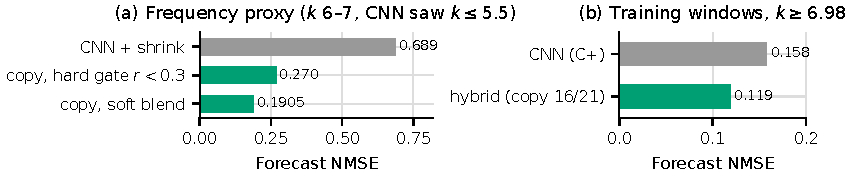
\includegraphics[width=\linewidth]{figures/fig3_period_copy.pdf}
\caption{Period copy, recorded results (per-window data not regenerated). (a) CNN
trained on $k\le5.5$, 132 held-out cases $k$ 6--7. (b) Training windows $k\ge6.98$,
real 10-frame history (copy NMSE 0.025 where used; CNN trained on these cases).}
\label{fig:copy}
\end{figure}

\section{Key insights}

\textbf{1. Symmetry helps once it is learned.} Test-time averaging
only pays off once the symmetry is learned. The organizer network never saw mirrored
inputs, so averaging blended a good forecast with a poor one; after mirror training
both passes were good with partly different errors, making averaging a free
two-model ensemble.
\par
\textbf{2. In-range accuracy came from training choices.} Overall \Ce{} $-$
A$_{\rm ref}$ $=-0.1390$ $[-0.1982,-0.0985]$, 12/12. The bottleneck was data and objective, not capacity:
using every training window and matching the loss to the metric gave the largest
gains almost for free; a wider network did not help, and ensembling added a final
increment.
\par\textbf{3. Extrapolation needs known physics, and validation cannot see it.} Most remaining hidden error lies outside the training range, where known
physics beats learning: the wake locks onto the known forcing period, so copying it
forward by whole periods works where the network has no data. Validation, entirely
in range, cannot register this gain.

\textbf{Beyond the score.} Consistency is not accuracy: A$_{\rm avg}$ has zero
defect and no measurable gain. Validation is blind to extrapolation: three of our
seven submissions share validation NMSE 0.1440 yet span portal scores 0.2876 to
0.1680. The out-of-range shrinkage partly games the metric: hedging toward the
history mean lowers squared error when the network is unreliable, but it blurs
vortices rather than predicting them, improving the score more than the physics. Clamping $k$ to the training range
made extrapolation worse (1.04 vs 0.99) and hiding $k$ in training did not help
(1.03--1.05): the value of $k$ is not the problem. Width 96 was worse than \Cn{} in
all 12 cases.

\section{Limitations \& next experiment}

One training seed and no matched no-augmentation control leave seed noise and the
effect of augmentation alone unmeasured. All decisions, including the ensemble
weight, used the same 12 validation cases, so validation numbers are optimistic. The
period copy covers only periodic, locked wakes at high frequency; amplitude
extrapolation remains unsolved. Next: give the period-copy forecast to the network as input channels to
correct; compare a Fourier neural operator~\citep{li2021} at equal budget; hold out
a $k$ band inside the training range to test clamping and shrinkage. \textbf{Takeaway for others:} before chasing validation gains, build a proxy from your
own training data that mimics the hidden shift (train on low frequencies, test on
high); that proxy, not validation, led us to the period copy.

\textbf{Prior work.} Wang et al.~\citep{wang2021} compare equivariant and augmented
fluid models; Elesedy and Zaidi~\citep{elesedy2021} prove group-averaging benefits under
assumptions that do not cover our clipped score; Fromme et al.~\citep{fromme2025} build
equivariance into the architecture. Our contribution is the measured comparison.

\section{Reproducibility, contributions \& AI use}

\textbf{Evidence.} One H100; SIDERIUS v1.1.0 (5ccb436f8), PyTorch 2.10/CUDA 12.8;
SIDERIUS master (e3163175) gives identical metrics. Data: train.npz only for fitting
(\href{https://doi.org/10.5281/zenodo.24386760}{doi:10.5281/zenodo.24386760}); seed 0;
released initialization (sha256 2bdf7cfd\dots), reproduced tensor-for-tensor by
\texttt{init -{}-seed 0}. Training: \texttt{run\_baseline.py train -{}-mirror
[-{}-loss nmse] -{}-train-only -{}-seed 0}; the \#129 command trains both networks and
merges them. A fresh 40-epoch reproduction matched B and C exactly; a smoke test of
the packaged C command reproduced B's epoch-0 loss (0.44678). The \#129 ZIP (sha256 853773018fb4\dots0c80c9106; source 469b3ce,
unchanged at head 269cd38) scores 0.118142 on validation when rerun on CPU.
Submissions \#52--\#129 rebind an internal $k$-range constant that the statistics
head also reads (fixed in 593c0aa): st\_abs\_error moves by $2.3\times10^{-5}$,
forecasts unchanged.
\href{https://github.com/pranavvkrishna/GalileoHackathon-Optimus}{Repository}.

\textbf{Contributions.} Pranav Vijay Krishna: repository, environment and SIDERIUS
setup; reflection transforms, augmentation and averaging code with unit tests; local
evaluator verified against the official scorer; training of B and B+; packages
C\_on\_A and C\_from\_B; pre-upload verification and all portal submissions. Raghav
Vijayakannan: gates and paired comparisons; extrapolation proxies; shrinkage, period
copy and soft blend; variance-normalised loss and ensemble; width-96 experiments;
packages \#52--\#129; report and figures. Hrithik Yash: shared-GPU scheduling; fresh
train-only reproduction matching B and C exactly; reproducibility evidence; report
review.

\textbf{AI use.} Claude Code (Anthropic) set up the environment, wrote and ran the
training patches, evaluation, gates, proxy experiments and packaging, and drafted
this report and figures; SIDERIUS provided the scorer and health checks; Codex and
Undermind supported earlier drafting and paper reading. We verified the reflection
transform (unit tests, physics review) and every number against saved outputs. AI drafted the factual sections and
figures; the research judgments, insights, limitations and conclusions were written
by the authors and only proofread by AI. Pranav verified every submission ZIP before
upload (files, manifest, weight sha256) and local scores against the official
scorer. All three authors read the final report; Pranav checked the submission table,
portal scores and reproducibility details against the portal and package hashes;
Raghav checked every quoted number against NUMBER\_SOURCES.md; Hrithik reviewed the
reflection-symmetry physics.

\clearpage
\begin{thebibliography}{9}

\bibitem{wang2021}
Rui Wang, Robin Walters, and Rose Yu.
Incorporating Symmetry into Deep Dynamics Models for Improved Generalization.
\emph{ICLR}, 2021.
\url{https://doi.org/10.48550/arXiv.2002.03061}.

\bibitem{elesedy2021}
Bryn Elesedy and Sheheryar Zaidi.
Provably Strict Generalisation Benefit for Equivariant Models.
\emph{Proceedings of ICML}, PMLR 139, 2021.
\url{https://doi.org/10.48550/arXiv.2102.10333}.

\bibitem{fromme2025}
Fynn Fromme, Christine Allen-Blanchette, Hans Harder, and Sebastian Peitz.
Surrogate Modeling of 3D Rayleigh--B\'enard Convection with Equivariant
Autoencoders. ArXiv preprint, 2025.
\url{https://doi.org/10.48550/arXiv.2505.13569}.

\bibitem{li2021}
Zongyi Li, Nikola Kovachki, Kamyar Azizzadenesheli, Burigede Liu, Kaushik
Bhattacharya, Andrew Stuart, and Anima Anandkumar.
Fourier Neural Operator for Parametric Partial Differential Equations.
\emph{ICLR}, 2021.
\url{https://doi.org/10.48550/arXiv.2010.08895}.

\end{thebibliography}
\end{document}
